\chapter{Das Induktionsprinzip}\label{ch:Kapitel02}

\cref{axiom:a5} wird \tib{Prinzip der vollständigen Induktion}\index{Prinzip der vollständigen Induktion} genannt. Dieses Kapitel wird sich mit diesem wichtigen Prinzip befassen.
Sie werden sehen, welche enorm weitreichenden Konsequenzen das \cref{axiom:a5} (Induktionsaxiom) der natürlichen Zahlen hat. Die Notation dieses Kapitels sowie einige Beweise stammen aus Kapitel 5 in \cite{AmannEscher1}.

\section{Einführende Beispiele}

\subsection{Teilbarkeit durch 2}
Ihre gute Freundin Anika behauptet, eine mathematische Entdeckung gemacht zu haben. Sie hat nämlich bemerkt, dass wenn zu dem Quadrat $n^2$ einer natürlichen Zahl $n$ die Zahl $n$ addiert wird, die entstandene Summe stets gerade ist. Sie behauptet also, dass für jede natürliche Zahl $n$ die Zahl $n^2+n$ gerade ist.

\begin{aufgabe}{aufgabe:0200}
Anika hat in der Vergangenheit schon öfters mathematische Behauptungen aufgestellt. Nicht selten haben sich diese bei genauerer Untersuchung als falsch erwiesen. Bevor Sie also viel Zeit in die genauere Analyse Anikas neuer Behauptung investieren, möchten Sie eine kurze \enquote{Plausibilitätsprüfung} durchführen. Schreiben Sie dazu ein Python-Programm, welches für die ersten $100$ natürlichen Zahlen $n\in\setcm{m\in\N}{0\leq m < 100}$ überprüft, ob $n^2+n$ jeweils gerade ist.
\end{aufgabe}
\begin{antwort}{aufgabe:0200}
\begin{lstlisting}[language=Python,caption=Vermutung überprüfen]
def vermutung(m):
    for n in range(m):
        if (n * n + n) % 2 != 0:
            return False
    return True

m = 100
print(vermutung(m))
\end{lstlisting}
\end{antwort}

\noindent
Das folgende Beispiel zeigt in aller Ausführlichkeit, wie das Prinzip der vollständigen Induktion verwendet werden kann, um eine mathematische Vermutung zu beweisen.

\beispiel{beispiel:InduktionEven}
{
Wir betrachten erneut die Vermutung Ihrer Freundin Anika:
\begin{center}
    Für jedes $n\in\N$ ist die Zahl $n^2+n$ gerade.
\end{center}
Wie lässt sich eine solche Vermutung überprüfen? Sicherlich können wir die Vermutung für einige natürliche Zahlen \enquote{von Hand} durch simples \enquote{Nachrechnen} überprüfen. In \cref{aufgabe:0200} haben Sie die Vermutung mit einem Computerprogramm für die ersten 100 natürlichen Zahlen überprüft. Das Problem ist jedoch, dass wir (selbst unter Verwendung von Supercomputern) immer nur endlich viele Zahlen überprüfen können. Wenn wir die Vermutung für 100 Milliarden Zahlen geprüft haben, bleiben immer noch unendlich viele Zahlen, die wir noch nicht betrachtet haben. Was wir benötigen, ist ein mathematisches Argument, welches grundsätzlich erklärt, warum die Vermutung stimmen muss. Ein solches mathematisches Argument liefert uns das Prinzip der vollständigen Induktion. Um dieses direkt anwenden zu können definieren wir die \enquote{Hilfsmenge}
\begin{align*}
    N:=\setct{n\in\N}{$n^2+n$ ist gerade}.
\end{align*}
Die so definierte Menge $N$ enthält genau die natürlichen Zahlen, für welche die Zahl $n^2+n$ gerade ist, für welche also die Vermutung gilt. Somit ist die Vermutung bewiesen, wenn wir nachweisen können, dass alle natürlichen Zahlen in $N$ liegen, dass also die Gleichheit $N=\N$ gilt. Es gilt somit:
\begin{center}
    (für jedes $n\in\N$ ist die Zahl $n^2+n$ gerade) $\quad\iff\quad$ ($N = \N$).
\end{center}
Nun besagt das Prinzip der vollständigen Induktion (\cref{axiom:a5}), dass für eine Teilmenge $N\subseteq\N$ tatsächlich $N=\N$ gilt, falls zwei Bedingungen erfüllt sind:
\begin{enumerate}
    \item $0\in N$,
    \item ist $n\in N$, dann enthält $N$ auch den Nachfolger $\nu(n) = n+1$.
\end{enumerate}
Wir prüfen diese beiden Bedingungen separat:
\begin{enumerate}
    \item In der Tat gilt $0\in N$, denn $0^2+0 = 0$ und $0$ ist gerade. \checkmark
    \item Sei $n\in N$ und somit $\textcolor{Green}{n^2+n}$ eine gerade Zahl. Wir müssen beweisen, dass auch $\nu(n)=(n+1)\in N$ gilt, dass also auch $(n+1)^2+(n+1)$ eine gerade Zahl ist. Dazu betrachten wir die folgende Berechnung:
    \begin{align*}
        (n+1)^2+(n+1) &= n^2+2n+1+(n+1) = n^2+3n+2 =\\
        n^2+n + (2n+2) &= \textcolor{Green}{n^2+n} + 2(n+1).
    \end{align*}
    Betrachten wir den Ausdruck $\textcolor{Green}{n^2+n} + 2(n+1)$. Wir wissen, dass die Zahl $\textcolor{Green}{n^2+n}$ gerade ist (da $n$ in der Menge $N$ liegt). Die Zahl $2(n+1)$ ist offensichtlich ebenfalls gerade. Somit ist $(n+1)^2+(n+1)$ als Summe zweier geraden Zahlen ebenfalls gerade. (Da die Zahl $n^2+n$ gerade ist, existiert eine natürliche Zahl $k$, sodass $n^2+n = 2k$. Dann ist die Summe $(n+1)^2+(n+1) = 2k + 2(n+1) = 2(k+n+1)$ das Doppelte der Zahl $k+n+1$ und somit gerade). \checkmark
\end{enumerate}
Damit sind die Bedingungen des Prinzips der vollständigen Induktion erfüllt und die Gleichheit $N = \N$ (und dadurch die ursprüngliche Vermutung Anikas) bewiesen.
}

\begin{aufgabe}{aufgabe:0299}
Verwenden Sie das Prinzip der vollständigen Induktion um zu beweisen, dass $n^5-n$ für jede natürliche Zahl $n$ durch $5$ teilbar ist.
\end{aufgabe}
\begin{antwort}{aufgabe:0299}
Wir definieren die \enquote{Hilfsmenge}
\begin{align*}
    N:=\setct{n\in\N}{$n^5-n$ ist durch $5$ teilbar}.
\end{align*}
Die Behauptung der Aufgabe ist bewiesen, wenn wir nachweisen können, dass alle natürlichen Zahlen in $N$ liegen, dass also die Gleichheit $N=\N$ gilt. Das Prinzip der vollständigen Induktion (\cref{axiom:a5}) besagt, dass für eine Teilmenge $N\subseteq\N$ tatsächlich $N=\N$ gilt, falls zwei Bedingungen erfüllt sind:
\begin{enumerate}
    \item $0\in N$,
    \item ist $n\in N$, dann enthält $N$ auch den Nachfolger $\nu(n) = n+1$.
\end{enumerate}
Wir prüfen nun diese beiden Bedingungen.
\begin{enumerate}
    \item In der Tat gilt $0\in N$, denn $0^5-0 = 0$ ist durch $5$ teilbar. \checkmark
    \item Sei $n\in N$ und somit $\textcolor{Green}{n^5-n}$ durch $5$ teilbar. Wir müssen beweisen, dass auch $\nu(n)=(n+1)\in N$ gilt, dass also auch $(n+1)^5-(n+1)$ durch $5$ teilbar ist. Dazu betrachten wir die folgende Berechnung:
    \begin{align*}
        (n+1)^5-(n+1) &= n^5+5n^4+10n^3+10n^2+5n+1-n-1 = \\
        &\lr{\textcolor{Green}{n^5-n}} + 5\lr{n^4+2n^3+2n^2+n}
    \end{align*}
    Da $n$ in der Menge $N$ liegt, ist die Zahl $\textcolor{Green}{n^5-n}$ durch $5$ teilbar. Somit ist $(n+1)^5-(n+1)$ als Summe zweier durch $5$ teilbarer Zahlen ebenfalls durch $5$ teilbar. \checkmark
\end{enumerate}
\end{antwort}

\subsection{Klingende Gläser}
In dem Gasthaus \textit{Inn of the Prancing Pony} stossen $n$ Gäste auf das neue Jahr an. Jede Person stösst mit jeder anderen (nicht mit sich selbst) genau einmal an. Wie viele Male klingen die Gläser (wie viele Male wird angestossen)? Die folgende elegante Überlegung, gibt uns eine Formel um die gesuchte Zahl rasch zu berechnen. Jede der $n$ Personen stösst offensichtlich mit genau $(n-1)$ Personen an (mit allen anderen). Damit klingen die Gläser also $n(n-1)$ mal. Die Formel ist so aber noch nicht richtig, denn wir haben jedes Klingen doppelt gezählt (anstatt nur einfach). Stösst nämlich Person $A$ mit Person $B$ an, dann haben wir dieses Anstossen einmal aus Sicht von $A$ gezählt und nochmal aus Sicht von $B$. Somit müssen wir die gesuchte Zahl $n(n-1)$ noch durch den Faktor 2 teilen. Die gesuchte Zahl ist also $n(n-1)/2$.
\beispiel{beispiel:InduktionGlases}
{
Diese Formel wollen wir nun mit Hilfe des Prinzips der vollständigen Induktion überprüfen. Dazu definieren wir, wie bereits in \cref{beispiel:InduktionEven}, die Behauptung in geeigneter Form. Für jedes $n\in\N$ definieren wir also die Aussage $\mathcal{A}(n)$ als
\begin{align*}
    &\mathcal{A}(n) :\iff \\
    &\text{Stossen $n$ Personen (alle mit allen)) an, klingen die Gläser genau } \frac{n(n-1)}{2} \text{ mal}.
\end{align*}
Um das Prinzip der vollständigen Induktion direkt anwenden zu können definieren wir erneut eine \enquote{Hilfsmenge} $N$ der Form
\begin{align*}
    N := \setct{n\in\N}{$\mathcal{A}(n)$ ist wahr}.
\end{align*}
Somit ist die Vermutung bewiesen, wenn wir nachweisen können, dass alle natürlichen Zahlen in $N$ liegen, dass also die Gleichheit $N=\N$ gilt. Erneut prüfen wir die beiden Bedingungen des Induktionsaxioms separat:
\begin{enumerate}
    \item Die behauptete Formel besagt, dass $n = 0$ Personen genau $0\cdot (0-1) = 0$ mal anstossen. Diese ist offensichtlich korrekt und somit haben wir $0\in N$ begründet. \checkmark
    \item Sei $n\in N$ und somit $\mathcal{A}(n)$ wahr. Wir müssen beweisen, dass auch $\nu(n)=(n+1)\in N$ gilt, dass also bei $(n+1)$ Personen genau $\textcolor{Red}{(n+1)n/2}$ mal die Gläser klingen. 
    
    \noindent
    Dazu stellen wir uns vor, dass erst $n$ Personen im Restaurant sind und diese bereits alle miteinander angestossen haben. Da $\mathcal{A}(n)$ wahr ist, wissen wir also, dass die Gläser bereits genau $\textcolor{Green}{n(n-1)/2}$ mal klangen. Nun kommt eine weitere Person hinzu. Diese Person stösst mit allen $\textcolor{Blue}{n}$ bereits anwesenden an. Damit klingen die Gläser genau $n$ weitere Male und insgesamt also
    \begin{align*}
        \textcolor{Green}{\frac{n(n-1)}{2}} + \textcolor{Blue}{n} = \frac{n(n-1)+2n}{2} = \frac{n(n-1+2)}{2} = \textcolor{Red}{\frac{(n+1)n}{2}}
    \end{align*}
    mal. \checkmark
\end{enumerate}
Somit ist die intuitiv gefundene Formel formal mit Hilfe des Prinzips der vollständigen Induktion nachgewiesen.}

\section{Erklimmen einer Leiter}
In \cref{beispiel:InduktionEven} und dem Beweis von \cref{satz:MinimumN} haben wir das Prinzip der vollständigen Induktion als Beweistechnik verwendet. Dabei haben wir jeweils auf geschickte Weise eine \enquote{Hilfsmenge} $N$ definiert und gezeigt, dass $N$ die Menge aller natürlichen Zahlen $\N$ ist. Nun möchten wir aber mathematische Aussagen beweisen und nicht unbedingt über Mengen sprechen. Deshalb ist es intuitiv einfacher, im Beweisverfahren der vollständigen Induktion, den Begriff der \textit{Menge} durch den Begriff der \textit{Aussage} zu ersetzen. Um dies konkreter zu machen, betrachten wir nochmals \cref{beispiel:InduktionEven}. In dem Beispiel kann man für jedes $n\in\N$ die Aussage $\mathcal{A}(n)$ definieren als
\begin{align*}
    \mathcal{A}(n) :\iff \text{Die Zahl $n^2 + n$ ist gerade}.
\end{align*}
In der Sprache der \textit{Aussagen} erhalten wir das folgende rezeptartige Beweisverfahren:
\begin{myBox}[Beweis durch vollständige Induktion]{mybox:Induktion}
Für jedes $n\in\N$ sei $\mathcal{A}(n)$ eine Aussage. Wir wollen beweisen, dass $\mathcal{A}(n)$ für jedes $n\in\N$ richtig ist. Der Beweis kann mit Hilfe des Prinzips der vollständigen Induktion erbracht werden, indem wie folgt vorgegangen wird:
\begin{aenum}
    \item \textit{Induktionsanfang}: Es wird gezeigt, dass $\mathcal{A}(0)$ richtig ist.
    \item \textit{Induktionsschluss}: Dieser besteht aus zwei Teilen:
        \begin{renum}
            \item \textit{Induktionsvoraussetzung}: Es sei $n$ eine natürliche Zahl und $\mathcal{A}(n)$ sei richtig.
            \item \textit{Induktionsschritt} ($n\to n+1)$: Man zeigt, dass aus der Induktionsvoraussetzung (i), logischen Schlüssen und bereits als wahr erkannter Aussagen die Richtigkeit von $\mathcal{A}(n+1)$ abgeleitet werden kann.
        \end{renum}
\end{aenum}
Damit ist die Richtigkeit von $\mathcal{A}(n)$ für alle $n\in\N$ gezeigt.
\end{myBox}
Beachten Sie, dass das Prinzip der vollständigen Induktion dem \cref{axiom:a5} entspricht und als solches nicht bewiesen werden kann. Was wir aber anbieten können, ist eine Metapher, welche das Prinzip veranschaulicht:
\begin{mdframed}[backgroundcolor=NavajoWhite!30,nobreak=true]\label{mdframed:Metapher}
\textbf{Metapher der Leiter}
\vspace{0.2cm}

\noindent
Die vollständige Induktion beweist, dass wir auf einer Leiter beliebig weit hochsteigen können, indem sie beweist, dass wir den untersten Tritt (Induktionsanfang) erreichen
können und, dass wir von jedem Tritt den nächst höheren erreichen können (Induktionsschluss).
\end{mdframed}

\begin{aufgabe}{aufgabe:0201}
Erklären Sie, wie das rezeptartige Beweisverfahren in \cref{mybox:Induktion} aus \cref{axiom:a5} folgt. Tipp: Definieren Sie die \enquote{Hilfsmenge}
\begin{align*}
    N := \setct{n\in\N}{$\mathcal{A}(n)$ ist richtig}
\end{align*}
aller natürlichen Zahlen, für welche $\mathcal{A}(n)$ richtig ist.
\end{aufgabe}
\begin{antwort}{aufgabe:0201}
Im \textit{Induktionsanfang} (a) wird gezeigt, dass $0\in N$ gilt. Der \textit{Induktionsschluss} liefert schliesslich, dass für $n\in N$ auch $(n+1)\in N$ gilt. Gemäss \cref{axiom:a5} gilt somit $N=\N$. Dies bedeutet aber, dass $\mathcal{A}(n)$ in der Tat für alle $n\in\N$ gilt.
\end{antwort}

\begin{aufgabe}{aufgabe:0202}
Beweisen Sie durch vollständige Induktion, dass für jede natürliche Zahl $n$ die Zahl $5^n-1$ durch $4$ teilbar ist.
\end{aufgabe}
\begin{antwort}{aufgabe:0202}
Für jedes $n\in\N$ definieren wir die Aussage $\mathcal{A}(n)$ als
\begin{align*}
    \mathcal{A}(n) :\iff \text{Die Zahl $5^n-1$ durch $4$ teilbar}.
\end{align*}
\begin{aenum}
    \item \textit{Induktionsanfang}: Wir zeigen, dass $\mathcal{A}(0)$ richtig ist. Dies ist aber klar, denn $5^0-1=0$ und $0$ ist durch $4$ teilbar.
    \item \textit{Induktionsschluss}:
        \begin{renum}
            \item \textit{Induktionsvoraussetzung}: Es sei $n$ eine natürliche Zahl und $\mathcal{A}(n)$ sei richtig. Sei also $5^n-1$ durch $4$ teilbar.
            \item \textit{Induktionsschritt} ($n\to n+1)$: Wir zeigen, dass aus der Induktionsvoraussetzung (i), logischen Schlüssen und bereits als wahr erkannter Aussagen die Richtigkeit von $\mathcal{A}(n+1)$ abgeleitet werden kann. Die Aussage $\mathcal{A}(n+1)$ lautet: $5^{n+1}-1$ ist durch $4$ teilbar. Wir berechnen:
            \begin{align*}
                5^{n+1}-1 = 5\cdot 5^{n}-1 = (4+1)\cdot 5^n - 1 = 4\cdot 5^n + \textcolor{Green}{5^n -1}.
            \end{align*}
            Die Zahl $4\cdot 5^n$ ist als Vielfaches von $4$, offensichtlich durch $4$ teilbar und $\textcolor{Green}{5^n -1}$ ist gemäss Induktionsvoraussetzung durch $4$ teilbar. Somit haben wir gezeigt, dass $5^{n+1}-1$ eine Summe von Termen ist, welche jeweils durch $4$ teilbar sind. Damit ist aber auch $5^{n+1}-1$ durch $4$ teilbar und der Induktionsschritt ist bewiesen.
        \end{renum}
\end{aenum}
Aus dem Induktionsprinzip folgt somit, dass $\mathcal{A}(n)$ für jedes $n\in\N$ korrekt ist.
\end{antwort}


\section{Zwei bedeutende Sätze über natürliche Zahlen (*!)}
Das Prinzip der vollständigen Induktion ist in der Mathematik und Informatik von enormer Bedeutung. Wir wollen in diesem anspruchsvollen Abschnitt noch mehr verdeutlichen, wie weitreichend die Beweiskraft dieses Prinzips ist. Dazu möchten wir zwei bedeutende Sätze der Mathematik besprechen und zeigen, wie diese aus dem Prinzip der vollständigen Induktion folgen.
\subsection{Wohlordnungsprinzip}
Beachten Sie, dass die Menge der ganzen Zahlen $\Z$ kein Minimum (kleinstes Element) besitzt. Zu jeder ganzen Zahl $m$ ist offensichtlich $m-1$ ebenfalls eine ganze Zahl, die (noch) kleiner ist als $m$. Die Teilmenge $\lrc{-3,-1,0,7}$ von $\Z$ hingegen besitzt $-3$ als Minimum.
\begin{definition}[ Minimum]{definition:min}
Es sei $A$ eine nichtleere Menge, in der sich Elemente durch die Relation $\leq$ vergleichen lassen. Ein Element $m\in A$ heisst \tib{Minimum}\index{Minimum} von $A$, falls
\begin{align*}
    m \leq x
\end{align*}
für alle $x\in A$ gilt. Das Minimum einer Menge $A$ muss selbst Element von $A$ sein. Beachten Sie, dass $A$ offensichtlich höchstens ein Minimum enthalten kann. Dieses wird mit $\min(A)$ bezeichnet.
\end{definition}

\begin{aufgabe}{aufgabe:0267}
\begin{aenum}
    \item Welches ist das Minimum von $\N$?
    \item Erklären Sie, warum das halboffene Intervall 
    \begin{align*}
        \ioc{0}{1} := \setcm{x\in\R}{0<x\leq 1}
    \end{align*}
    kein Minimum besitzt.
\end{aenum}
\end{aufgabe}
\begin{antwort}{aufgabe:0267}
    \begin{aenum}
        \item Die Zahl $0$ ist das Minimum von $\N$, da $0\in\N$ und $0\leq x$ für alle $x\in\N$.
        \item Für jedes Element $m\in\ioc{0}{1}$ ist auch die Hälfte $m/2$ von $m$ Element des Intervalls. Dann gilt aber auch $\lr{m/2}\in\ioc{0}{1}$. Anders gesagt: Angenommen $m\in\ioc{0}{1}$ sei das Minimum des Intervalls. Dann gilt aber auch $\lr{m/2}\in\ioc{0}{1}$. Wegen $m/2<m$ ist dies aber ein Widerspruch zur Minimalität von $m$.
    \end{aenum}
\end{antwort}
Wir haben gesehen, dass durchaus nicht jede Menge ein Minimum besitzt. Das sogenannte \tib{Wohlordnungsprinzip}\index{Wohlordnungsprinzip} der natürlichen Zahlen garantiert uns aber, dass jede Teilmenge von $\N$, welche nicht die leere Menge ist, ein Minimum besitzt. Die leere Menge besitzt keine Elemente und somit offensichtlich auch kein minimales Element. Weshalb ist das Wohlordnungsprinzip für uns interessant? Dieses Prinzip kommt in den Beweisen einiger wichtiger mathematischen Behauptungen zum Einsatz. So zum Beispiel in unserem Beweis des berühmten \textit{Fundamentalsatzes der Arithmetik}, den wir in \cref{subsec:fundamental} besprechen.

\begin{definition}[untere Schranke]{definition:schranke}
Seien $D$ eine Menge und $A\subseteq D$ eine nichtleere Teilmenge von $D$. Jedes Element $s\in D$, welches $s \leq a$ für alle $a\in A$ erfüllt, heisst \tib{untere Schranke}\index{untere Schranke} von $A$. Eine untere Schranke von $A$ muss selbst nicht ein Element von $A$ sein.   
\end{definition}
\noindent
Wir erkennen nun: Ein Element $m\in\R$ heisst \textit{Minimum} von $A\in\R$, falls $m$ eine untere Schranke von $A$ ist und zusätzlich $m\in A$ gilt.

\beispiele{-}{}
{Die Zahlen $-5, 0, 3, 4$ sind Beispiele von unteren Schranken der Menge $A:=\lrc{4,7,9,18}$. Da $4\in A$ und $4$ eine untere Schranke von $A$ ist, gilt
\begin{align*}
    \min(A) = 4.
\end{align*}
}
{Die Menge $\Z$ der ganzen Zahlen besitzt keine untere Schranke.}

\begin{aufgabe}{aufgabe:0298}
Welches ist die grösste untere Schranke des halboffenen Intervalls
    \begin{align*}
        \ioc{0}{1} := \setcm{x\in\R}{0<x\leq 1}?
    \end{align*}
\end{aufgabe}
\begin{antwort}{aufgabe:0298}
Das halboffene Intervall $\ioc{0}{1} := \setcm{x\in\R}{0<x\leq 1}$ besitzt die grösste untere Schranke $0$, aber kein Minimum.
\end{antwort}

\begin{aufgabe}{aufgabe:0297}
    \begin{aenum}
        \item Sei $A\subseteq\N$ eine Teilmenge der natürlichen Zahlen. Angenommen $n\in\N$ sei eine untere Schranke von $A$, wobei aber $n$ selbst nicht Element der Menge $A$ ist ($n$ ist also nicht das Minimum von $A$). Begründen Sie, warum auch der Nachfolger $n+1$ eine untere Schranke von $A$ ist.
        \item Sei $A\subseteq\N$ eine Teilmenge der natürlichen Zahlen mit der Eigenschaft, dass jede natürliche Zahl eine untere Schranke von $A$ ist. Beweisen Sie, dass $A$ die leere Menge ist. Tipp: Nehmen Sie an, $A$ sei nichtleer. Dann enthält $A$ also (zumindest) ein Element $m\in A$. Betrachten Sie nun die natürliche Zahl $m+1$.
    \end{aenum}
    \end{aufgabe}
    \begin{antwort}{aufgabe:0297}
    \begin{aenum}
        \item Da $n$ eine untere Schranke von $A$ ist, gilt $n\leq a$ für alle $a\in A$. Da aber $n\notin A$, ist klar, dass tatsächlich sogar $n < a$ (echt kleiner) für alle $a\in A$ gilt. Der Nachfolger (die nächst grössere natürliche Zahl) von $n$ ist $n+1$. Damit ist klar, dass $n+1$ höchstens so gross wie jedes der Elemente in $A$ ist, dass also $n+1 \leq a$ für alle $a\in A$ gilt.
        \item Angenommen $A$ wäre nichtleer. Dann enthält $A$ mindestens ein Element $m\in A$. Die natürliche Zahl $m+1$ ist grösser als $m\in A$ und somit keine untere Schranke von $A$. Doch $A$ besitzt die Eigenschaft, dass jede natürliche Zahl eine untere Schranke von $A$ ist. Dies ist ein Widerspruch und somit muss $A$ die leere Menge sein.
    \end{aenum}
\end{antwort}

\noindent
Wir verwenden nun das Prinzip der vollständigen Induktion, um das \textit{Wohlordnungsprinzip} zu beweisen. Wir haben den Beweis dieses Satzes inzwischen recht gut vorbereitet. Dennoch ist der Beweis recht anspruchsvoll! Nehmen Sie sich Zeit um die einzelnen Schritte zu studieren.
\begin{satz}[Wohlordnungsprinzip]{satz:MinimumN}
{Jede nichtleere Teilmenge der natürlichen Zahlen besitzt ein Minimum.}
\end{satz}
\beweis{
Wir beweisen den Satz durch Widerspruch. Angenommen eine Teilmenge $A\subseteq\N$ sei \textbf{nichtleer} und besitze \textbf{kein Minimum}. Dann definieren wir zu $A$ die \enquote{Hilfsmenge}
\begin{align*}
    N := \setct{n\in\N}{$n$ ist untere Schranke von $A$}
\end{align*}
aller unteren Schranken von $A$. Mit dem Prinzip der vollständigen Induktion beweisen wir, dass jede natürliche Zahl eine untere Schranke von $A$ ist, dass also $N=\N$ gilt. In \cref{aufgabe:0298} haben Sie bereits bewiesen, dass dies nur möglich ist, falls $A$ die leere Menge ist. Um $N = \N$ durch die vollständige Induktion zu beweisen, müssen wir, wie immer, zwei Bedingungen prüfen:
\begin{enumerate}
    \item $0\in N$,
    \item Ist $n\in N$, dann enthält $N$ auch den Nachfolger $\nu(n) = n+1$ von $n$. \textcolor{Gray}{(Ist $n$ eine untere Schranke von $A$, dann ist auch $n+1$ eine untere Schranke von $A$.)}
\end{enumerate}
Wir prüfen diese beiden Bedingungen separat:
\begin{enumerate}
    \item $0$ ist die kleinste Zahl in $\N$ und somit gilt $0\leq a$ für jedes Element $a\in A$. Damit ist $0$ eine untere Schranke von $A$ und wir haben $0\in N$ gezeigt. \checkmark
    \item Es sei $n\in N$ und somit $n$ eine untere Schranke von $A$. Beachten Sie, dass $n$ nicht in $A$ liegt, denn sonst würde die Menge $A$ die Zahl $n$ als ihr Minimum besitzen (doch $A$ besitzt gemäss Annahme kein Minimum). Damit ist $n\in\N$ eine untere Schranke von $A$, wobei aber $n$ selbst nicht Element der Menge $A$ ist. In \cref{aufgabe:0297} haben Sie gezeigt, dass dann auch $n+1$ eine untere Schranke von $A$ und somit ein Element von $N$ ist. \checkmark
\end{enumerate}
Aus dem Prinzip der vollständigen Induktion folgt nun, dass $N=\N$ gilt. Also ist jede natürliche Zahl eine untere Schranke von $A$. Somit ist $A\subseteq\N$ eine Teilmenge der natürlichen Zahlen mit der Eigenschaft, dass jede natürliche Zahl eine untere Schranke von $A$ ist. In \cref{aufgabe:0297} haben Sie gezeigt, dass $A$ somit die leere Menge ist. Damit haben wir den gewünschten Widerspruch $A\neq\emptyset$ und $A=\emptyset$ gefunden. Somit besitzt jede nichtleere Teilmenge von $\N$ ein Minimum.}

\subsection{Fundamentalsatz der Arithmetik}\label{subsec:fundamental}
Die Tatsache, dass jede Teilmenge der natürlichen Zahlen ein Minimum besitzt, erlaubt uns, den berühmten \textit{Fundamentalsatz der Arithmetik} zu beweisen.
\begin{satz}[Fundamentalsatz der Arithmetik (Primfaktorzerlegung)]{satz:Fundamentalsatz}
Ausser $0$ und $1$ kann jede natürliche Zahl als Produkt endlich vieler Primzahlen dargestellt werden. Diese Darstellung ist bis auf die Reihenfolge der Faktoren eindeutig und wird \textit{Primfaktorzerlegung} genannt. Erlaubt sind auch Produkte, die nur aus einem Faktor bestehen.
\end{satz}
\beispiele{-}{}
{Die Zahl $63$ besitzt die Primfaktorzerlegung $63 = 3\cdot 3\cdot 7$ und die Zahl $286$ die Darstellung $286 = 2\cdot 11\cdot 13$.}
{Die Primfaktorzerlegung der Primzahl $19$ ist $19$ selbst. Sie besteht also aus dem Produkt mit nur dem einen Faktor $19$. Jede Primzahl $p$ ist also bereits in Primfaktoren zerlegt.}

\beweis{Wir wollen nun den Fundamentalsatz (\cref{satz:Fundamentalsatz}) beweisen. Dies tun wir unter der Verwendung des Wohlordnungsprinzips. Allerdings zeigen wir nur, dass immer eine Zerlegung in Primfaktoren existiert. Auf den Beweis der Eindeutigkeit verzichten wir an dieser Stelle.

Angenommen die Behauptung sei falsch. Dann gibt es eine natürliche Zahl $\geq 2$, welche keine Primfaktorzerlegung besitzt. Mit anderen Worten: Die Menge
\begin{align*}
    A := \setct{n\in\N}{$n\geq 2$ und $n$ besitzt keine Primfaktorzerlegung}
\end{align*}
ist \textbf{nichtleer}. Dann liegt in $A$ aber gemäss \cref{satz:MinimumN} eine kleinste Zahl $n_0\geq 2$, welche nicht in Primfaktoren zerlegt werden kann. Insbesondere ist $n_0$ keine Primzahl. Da $n_0$ keine Primzahl ist, existieren natürliche Zahlen $n$ und $m$, sodass $n_0=n\cdot m$ und $n,m>1$. Es ist klar, dass die Faktoren $n$ und $m$ jeweils kleiner als das Produkt $n_0$ sind. Da aber $n_0$ die kleinste natürliche Zahl ist, welche keine Primfaktorzerlegung besitzt, können sowohl $n$ als auch $m$ jeweils als Produkt endlich vieler Primzahlen geschrieben werden. Dann ist aber auch $n_0$ als Produkt von $n$ und $m$ ein Produkt endlich vieler Primzahlen. Dieses Produkt wäre denn aber eine Primfaktorzerlegung von $n_0$. Das ist ein Widerspruch.}


\begin{aufgabe}{aufgabe:0293}
Die Zahl $30031$ lässt sich als Produkt
\begin{align*}
    30031 = p_1p_2
\end{align*}
zweier verschiedener Primfaktoren $p_1$ und $p_2$ schreiben. Schreiben Sie ein Python-Programm, welches $p_1$ und $p_2$ berechnet.
\end{aufgabe}
\begin{antwort}{aufgabe:0293}
\begin{lstlisting}[language=Python]
n = 30031
for k in range(2,n):
    if (n % k == 0):
        p1 = k
        break
p2 = int(n / p1)
print(n,'=', p1, '*',p2)
\end{lstlisting}
\end{antwort}


\begin{aufgabe}{aufgabe:0292}
Der griechische Mathematiker \textit{Euklid von Alexandria} bewies bereits im 3. Jahrhundert v. Chr., dass unendlich viele Primzahlen existieren. Dazu nahm er (indirekter Beweis) an, die Menge $P$ aller Primzahlen sei endlich. Wir können $P$ also schreiben als
\begin{align*}
    P = \lrc{p_1, p_2, p_3, \ldots , p_n}.
\end{align*}
Nun betrachtete Euklid das Produkt dieser $n$ Primzahlen und addierte dazu $1$:
\begin{align*}
    m := p_1\cdot p_2\cdot p_3\cdot \ldots \cdot p_n + 1.
\end{align*}
Betrachten Sie die so entstandene Zahl $m$. Welche Eigenschaften hat $m$ gemäss unseren Annahmen? Vervollständigen Sie den Beweis.
\end{aufgabe}
\begin{antwort}{aufgabe:0292}
Da $m\geq 2$ ist, lässt sich $m$ gemäss \cref{satz:Fundamentalsatz} als Produkt von Primzahlen schreiben. Für jeden Primteiler $p$ von $m$ gilt $p\neq p_i$ für alle $i=1,2,\ldots , n$. Es gibt also eine weitere Primzahl $p\notin P$. Dies ist ein Widerspruch zur Annahme, dass $P$ alle Primzahlen enthält.
\end{antwort}

\bemerkung{-}{Beachten Sie, dass das Vorgehen in \cref{aufgabe:0292} in keinster Weise ein Rezept zur Konstruktion von Primzahlen liefert. Beispielsweise gilt
\begin{align*}
    2\cdot 3\cdot 5\cdot 7\cdot 11\cdot 13 + 1 = 30031,
\end{align*}
doch Sie haben in \cref{aufgabe:0293} bereits gezeigt, dass $30031$ keine Primzahl ist.
}

\clearpage
\section{Leicht verallgemeinertes Induktionsprinzip}
Wie Sie sofort nachprüfen können, ist die mathematische Aussage $n^2 - 2n - 1 > 0$ für die natürlichen Zahlen $n = 0, 1, 2$ falsch. Nun möchten Sie aber beweisen, dass die Aussage für alle $n\in\N$ mit $n\geq 3$ gilt. Unser Beweisverfahren in \cref{mybox:Induktion} muss also dahingehend angepasst werden, dass es uns auch erlaubt, den Induktionsanfang bei einer beliebigen Zahl $n_0\in\N$ anzusetzen, wobei $n_0$ auch grösser als $0$ sein darf. Diese sehr geringfügige (aber wichtige) Verallgemeinerung fassen wir in dem folgenden Satz zusammen:
\begin{satz}[(leicht verallgemeinertes) Induktionsprinzip]{satz:n0Induktion}
Sei $n_0\in\N$ und für jedes $n\in\N$ mit $n\geq n_0$ sei $\mathcal{A}(n)$ eine Aussage. Zudem gelte:
\begin{renum}
    \item $\mathcal{A}\lr{n_0}$ ist richtig.
    \item Für jede Zahl $n\in\N$ mit $n\geq n_0$ folgt aus der Richtigkeit von $\mathcal{A}(n)$ die Richtigkeit von $\mathcal{A}(n+1)$.
\end{renum}
Dann ist $\mathcal{A}(n)$ für jedes $n\geq n_0$ richtig.
\end{satz}
\beweis{Der Beweis ist fast komplett analog zu der Begründung in \cref{aufgabe:0201}. Der einzige Unterschied besteht darin, dass wir einen Index \enquote{verschieben} müssen. Intuitiv gesprochen, möchten wir, dass wir immer noch bei $0$ beginnen, anstelle von $\mathcal{A}(0)$ aber bereits $\mathcal{A}\lr{n_0}$ betrachten. Wir definieren also die Menge $N$ der um \enquote{$\textcolor{Red}{n_0}$ verschobenen Aussagen}
\begin{align*}
    N := \setct{n\in\N}{$\mathcal{A}\lr{n+\textcolor{Red}{n_0}}$ ist richtig}.
\end{align*}
Beachten Sie, dass für $n=0$ dadurch bereits die Aussage $\mathcal{A}\lr{0+n_0}=\mathcal{A}\lr{n_0}$ gemeint ist. Mit dem Induktionsaxiom \ref{axiom:a5} folgt sofort $N=\N$ und somit ist $\mathcal{A}(n)$ für jedes $n\geq n_0$ richtig.}

\bemerkung{-}{
Wir werden das leicht verallgemeinerte Induktionsprinzip von \cref{satz:n0Induktion} ebenfalls einfach nur \textit{Induktionsprinzip} nennen.
}

\section{Übungsaufgaben zum Induktionsprinzip}

\begin{aufgabe}{aufgabe:0204}
Setzen Sie $n_0 := 3$ und beweisen Sie die Korrektheit der Ungleichung $n^2 - 2n - 1 > 0$ für alle $n\in\N$ mit $n\geq n_0$ mittels vollständiger Induktion.
\end{aufgabe}

\begin{antwort}{aufgabe:0204}
Für jedes $n\in\N$ mit $n\geq n_0$ definieren wir die Aussage $\mathcal{A}(n)$ als
\begin{align*}
    \mathcal{A}(n) :\iff n^2-2n-1 > 0.
\end{align*}
\begin{aenum}
    \item \textit{Induktionsanfang}: Wir zeigen, dass $\mathcal{A}(n_0)$ richtig ist. Für $n=3$ ist
    \begin{align*}
        n^2-2n-1 = 9-6-1 = 2 > 0.
    \end{align*}
    Somit stimmt die Aussage für $n=3$.
    \item \textit{Induktionsschluss}:
        \begin{renum}
            \item \textit{Induktionsvoraussetzung}: Es sei $n\geq n_0$ eine natürliche Zahl und $\mathcal{A}(n)$ sei richtig. Sei also
            \begin{align*}
                \textcolor{Green}{n^2-2n-1} > 0.
            \end{align*}
            \item \textit{Induktionsschritt} ($n\to n+1)$: Wir schreiben die Aussage $\mathcal{A}(n+1)$ explizit hin:
            \begin{align*}
                \textcolor{Red}{(n+1)^2-2(n+1)-1} > \textcolor{Red}{0}.
            \end{align*}
            Beweis des Induktionsschritts:
            \begin{align*}
                &\textcolor{Red}{(n+1)^2-2(n+1)-1} = n^2 + 2n + 1 - 2n - 2 - 1 = \\
                &\textcolor{Green}{n^2-2n-1} + 2n+1-2 = \textcolor{Green}{n^2-2n-1} + 2n-1 \stackrel{\text{Induktionsvoraussetzung}}{>}\\
                &2n-1 > \textcolor{Red}{0}.
            \end{align*}
        Beachten Sie, dass für $n\geq 0$ der Term $2n-1$ grösser als $0$ ist.
        \end{renum}
\end{aenum}
Mit \cref{satz:n0Induktion} folgt, dass $\mathcal{A}(n)$ für jedes $n\in\N$ mit $n\geq 3$ korrekt ist.
\end{antwort}

\begin{aufgabe}{aufgabe:0205}
Sie vermuten, dass die Zahl $n^3-n$ für jede natürliche Zahl $n\geq 2$ durch $3$ teilbar ist. Beweisen Sie diese Behauptung durch vollständige Induktion. Finden Sie auch einen direkten Beweis (welcher nicht das Induktionsprinzip verwendet)? Tipp für den direkten Beweis: Schreiben Sie die Zahl $n^3-n$ als Produkt dreier Faktoren.
\end{aufgabe}

\begin{antwort}{aufgabe:0205}
Die Behauptung lässt sich sehr elegant direkt beweisen, wenn man die Zahl $n^3-n$ als das Produkt
\begin{align*}
    n^3-n = (n-1)n(n+1)
\end{align*}
von drei Faktoren schreibt. Da die drei Zahlen $(n-1), n$ und $(n+1)$ direkt aufeinander folgen, muss genau eine von ihnen durch $3$ teilbar sein. Damit besitzt aber mindestens ein Faktor den Teiler $3$. Somit ist das Produkt $(n-1)n(n+1)$ und dadurch auch $n^3-n$ durch $3$ teilbar. Dies stellt einen direkten Beweis der Aussage dar.

Nun beweisen wir die Aussage auch durch vollständige Induktion. Für jedes $n\in\N$ mit $n\geq 2$ definieren wir die Aussage $\mathcal{A}(n)$ als
\begin{align*}
    \mathcal{A}(n) :\iff \text{Die Zahl } n^3-n \text{ ist durch $3$ teilbar}.
\end{align*}
\begin{aenum}
    \item \textit{Induktionsanfang}: Wir zeigen, dass $\mathcal{A}(2)$ richtig ist. Für $n=2$ ist
    \begin{align*}
        n^3-n = 2^3-2 = 6
    \end{align*}
    und $6$ ist durch $3$ teilbar. Somit stimmt die Aussage für $n=2$.
    \item \textit{Induktionsschluss}:
        \begin{renum}
            \item \textit{Induktionsvoraussetzung}: Es sei $n\geq n_0$ eine natürliche Zahl und $\mathcal{A}(n)$ sei richtig. Sei also $\textcolor{Green}{n^3-n}$ durch $3$ teilbar.
            \item \textit{Induktionsschritt} ($n\to n+1)$:
            \begin{align*}
                & (n+1)^3-(n+1) = \\
                & n^3+3n^2+3n+1 - (n+1) = \\
                & n^3+3n^2+2n = \\
                & n^3-n+3n^2+3n = \\
                & \underbrace{\textcolor{Green}{n^3-n}}_{\text{Induktionsvoraussetzung}}+\underbrace{3(n^2+n)}_{\text{ganzzahliges Vielfaches von $3$}}
            \end{align*}
        Der erste Summand ist nach Induktionsvoraussetzung durch $3$ teilbar. Der zweite Summand ist als ganzzahliges Vielfaches von $3$ ebenfalls durch $3$ teilbar. Damit ist die Aussage auch für $n+1$ erfüllt.
        \end{renum}
\end{aenum}
Mit \cref{satz:n0Induktion} folgt, dass $\mathcal{A}(n)$ für jedes $n\in\N$ mit $n\geq 2$ korrekt ist.
\end{antwort}

\begin{aufgabe}[Bernoullische Ungleichung]{aufgabe:0206}
Es sei $x\in\R$ mit $x\geq -1$ eine reelle Zahl. Für jede natürliche Zahl $n$ gilt die Bernoullische Ungleichung $(1+x)^n\geq 1+nx$.
\begin{figure}[H]
    \centering
    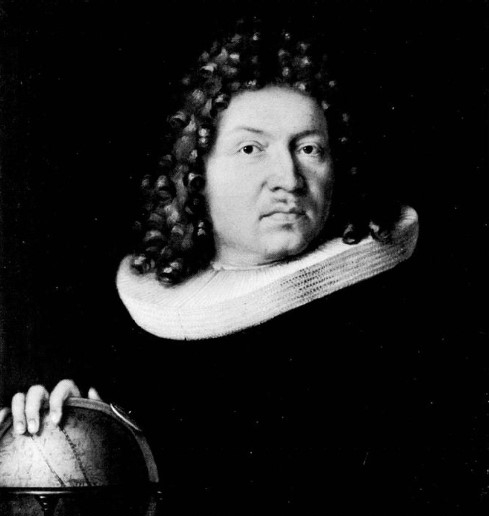
\includegraphics[width=0.20\textwidth]{Bernoulli.jpg}
    \caption{Jakob I Bernoulli (1654-1705) war ein Schweizer Mathematiker und Mitglied der angesehenen Gelehrtenfamilie Bernoulli.}
    \label{fig:Bernoulli}
\end{figure}
\end{aufgabe}
\begin{antwort}{aufgabe:0206}
Es sei $x\in\R$ mit $x\geq -1$ eine reelle Zahl. Für jedes $n\in\N$ definieren wir die Aussage $\mathcal{A}(n)$ als
\begin{align*}
    \mathcal{A}(n) :\iff (1+x)^n\geq 1+nx.
\end{align*}
\begin{aenum}
    \item \textit{Induktionsanfang}: Wir zeigen, dass $\mathcal{A}(0)$ richtig ist. Für $n=0$ ist
    \begin{align*}
        (1+x)^0 = 1 \geq 1 + 0\cdot x = 1.
    \end{align*}
    Somit stimmt die Aussage für $n=0$.
    \item \textit{Induktionsschluss}:
        \begin{renum}
            \item \textit{Induktionsvoraussetzung}: Es sei $n\geq n_0$ eine natürliche Zahl und $\mathcal{A}(n)$ sei richtig. Sei also
            \begin{align*}
                \textcolor{Green}{(1+x)^n} \geq \textcolor{Blue}{1+nx}.
            \end{align*}
            \item \textit{Induktionsschritt} ($n\to n+1)$: Wir schreiben die Aussage $\mathcal{A}(n+1)$ explizit hin:
            \begin{align*}
                \textcolor{Red}{(1+x)^{n+1}} \geq \textcolor{Red}{1 + (n+1)x}.
            \end{align*}
            Beweis des Induktionsschritts:
            \begin{align*}
                &\textcolor{Red}{(1+x)^{n+1}} = \textcolor{Green}{(1+x)^n} (1+x) \stackrel{\text{Induktionsvoraussetzung und }(1+x)\geq 0}{\geq}\\
                &\textcolor{Blue}{(1+nx)}(1+x) = 1+x+nx+nx^2 = 1+(n+1)x + nx^2 \stackrel{(nx^2)\geq 0}{\geq}\\
                &\textcolor{Red}{1 + (n+1)x}.
            \end{align*}
        Doch dies ist genau die Behauptung $\mathcal{A}(n+1)$.
        \end{renum}
\end{aenum}
Aus dem Induktionsprinzip folgt somit, dass $\mathcal{A}(n)$ für jedes $n\in\N$ korrekt ist.
\end{antwort}

\begin{aufgabe}{aufgabe:0207}
(*!) In die Ebene wurden $n\in\N$ verschiedene Geraden gelegt. Die Geraden teilen die Ebene in verschiedene Bereiche. Wir sagen, dass zwei Bereiche \textit{benachbart} sind, falls sie sich eine (möglicherweise unendlich lange) Grenzlinie teilen. Falls zwei Bereiche lediglich einen Grenzpunkt teilen (keine Grenzlinie), sind sie nicht benachbart.

Wir haben zwei Farben zur Verfügung und müssen jeden Bereich mit genau einer dieser Farben einfärben. Eine Färbung wird \textit{zulässig} genannt, falls zusätzlich keine zwei benachbarten Bereiche mit derselben Farbe gefärbt wurden. In \cref{fig:2lines} ist eine mögliche zulässige Färbung für zwei Geraden ($n=2$) gezeigt.

Skizzieren Sie eine zulässige Färbung für $n=3$ für den Fall, dass sich alle drei Geraden jeweils gegenseitig schneiden. Beweisen Sie anschliessend durch vollständige Induktion, dass es immer möglich ist, die verschiedenen Bereiche mit nur zwei Farben so zu färben, dass keine zwei benachbarten Bereiche von derselben Farbe sind.

% 2 lines
\begin{figure}[H]
    \centering
    \begin{subfigure}{0.4\textwidth}
        \centering
        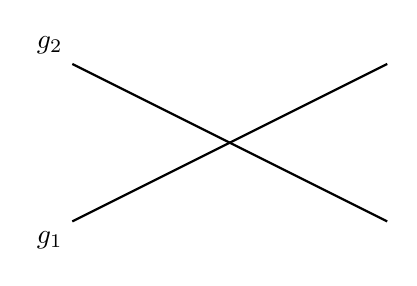
\begin{tikzpicture}[scale=0.50]
            \colorlet{c1}{Gold}
            \colorlet{c2}{CornflowerBlue}
    
            \coordinate (A1) at (-4,-2);
            \coordinate (A2) at (4,2);
            \coordinate (B1) at (-4,2);
            \coordinate (B2) at (4,-2);
            
            \node[below left] at (A1) {$g_1$};
            \node[above left] at (B1) {$g_2$};
            
            \foreach \k in {A,B}
                \draw[black, thick] (\k1) -- (\k2);
        \end{tikzpicture}
        \caption{zwei sich schneidende Geraden}
        \label{subfig:2linesNotFilled}
    \end{subfigure}
    \hfill
    \begin{subfigure}{0.4\textwidth}
        \centering
        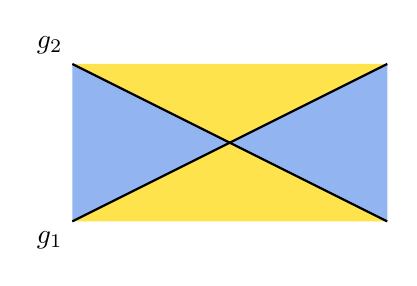
\begin{tikzpicture}[scale=0.50]
            \colorlet{c1}{Gold}
            \colorlet{c2}{CornflowerBlue}
    
            \coordinate (A1) at (-4,-2);
            \coordinate (A2) at (4,2);
            \coordinate (B1) at (-4,2);
            \coordinate (B2) at (4,-2);
            
            \node[below left] at (A1) {$g_1$};
            \node[above left] at (B1) {$g_2$};
            
            \coordinate (X) at (intersection cs:first line={(A1)--(A2)}, second line={(B1)--(B2)});
            
            \fill[c1,opacity=0.7]
                (A1) -- (X) -- (B2);
            \fill[c1,opacity=0.7]
                (B1) -- (X) -- (A2);
            \fill[c2,opacity=0.7]
                (A1) -- (X) -- (B1);
            \fill[c2,opacity=0.7]
                (A2) -- (X) -- (B2);
            \foreach \k in {A,B}
                \draw[black, thick] (\k1) -- (\k2);
        \end{tikzpicture}
        \caption{zulässige Färbung für $n=2$}
        \label{subfig:2linesFilled}
    \end{subfigure}
    \caption{Beispiel einer zulässigen Färbung für $n=2$. Beachten Sie, dass die beiden \textcolor{Gold}{goldenen} Bereiche sich nur einen Grenzpunkt (keine Grenzlinie) teilen und somit nicht benachbart sind. Das Gleiche gilt für die beiden \textcolor{CornflowerBlue}{blauen} Bereiche. Zwei sich schneidende Geraden teilen die Ebene in vier Bereiche ein. Zwei parallele Geraden teilen die Ebene in drei Bereiche ein.}
    \label{fig:2lines}
\end{figure}
\end{aufgabe}

\begin{antwort}{aufgabe:0207}
In \cref{fig:3lines} ist eine zulässige Färbung für drei Geraden skizziert.
% 3 lines
\begin{figure}[H]
    \centering
     \begin{subfigure}[b]{0.45\textwidth}
        \centering
        \begin{tikzpicture}[scale=0.7]
            \colorlet{c1}{Gold}
            \colorlet{c2}{CornflowerBlue}
            
            \coordinate (A1) at (-2,-2);
            \coordinate (A2) at (2,3);
            \coordinate (B1) at (-3,0);
            \coordinate (B2) at (5,0);
            \coordinate (C1) at (-1,3);
            \coordinate (C2) at (5,-2);
            
            \node[below left] at (A1) {$g_1$};
            \node[left] at (B1) {$g_2$};
            \node[above left] at (C1) {$g_3$};
            
            \foreach \k in {A,B,C}
                \draw[black, thick] (\k1) -- (\k2);
        \end{tikzpicture}
        \caption{Drei verschiedene Geraden $g_1, g_2$ und $g_3$ teilen die Ebene in sieben Bereiche ein.}
        \label{subfig:3linesNotFilled}
    \end{subfigure}
    \begin{subfigure}[b]{0.45\textwidth}
        \centering
        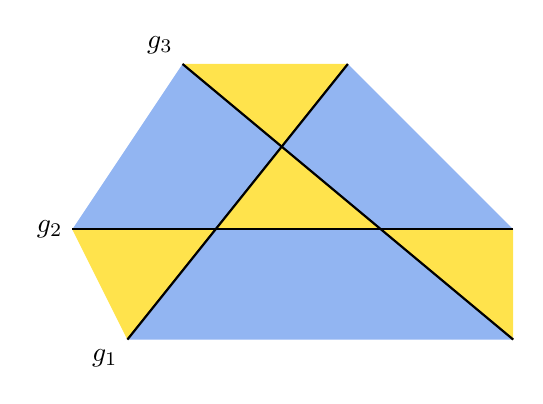
\begin{tikzpicture}[scale=0.7]
            \colorlet{c1}{Gold}
            \colorlet{c2}{CornflowerBlue}
            
            \coordinate (A1) at (-2,-2);
            \coordinate (A2) at (2,3);
            \coordinate (B1) at (-3,0);
            \coordinate (B2) at (5,0);
            \coordinate (C1) at (-1,3);
            \coordinate (C2) at (5,-2);
            
            \node[below left] at (A1) {$g_1$};
            \node[left] at (B1) {$g_2$};
            \node[above left] at (C1) {$g_3$};
            
            \coordinate (X) at (intersection cs:first line={(A1)--(A2)}, second line={(B1)--(B2)});
            \coordinate (Y) at (intersection cs:first line={(A1)--(A2)}, second line={(C1)--(C2)});
            \coordinate (Z) at (intersection cs:first line={(B1)--(B2)}, second line={(C1)--(C2)});
            
            \fill[c1,opacity=0.7]
                (A1) -- (X) -- (B1);
            \fill[c1,opacity=0.7]
                (A2) -- (Y) -- (C1);
            \fill[c1,opacity=0.7]
                (B2) -- (Z) -- (C2);
            \fill[c1,opacity=0.7]
                (X) -- (Y) -- (Z);
        
            \fill[c2,opacity=0.7]
                (A1) -- (X) -- (Z) -- (C2);
            \fill[c2,opacity=0.7]
                (B1) -- (X) -- (Y) -- (C1);
            \fill[c2,opacity=0.7]
                (A2) -- (Y) --(Z) -- (B2);
            
            \foreach \k in {A,B,C}
                \draw[black, thick] (\k1) -- (\k2);
        \end{tikzpicture}
        \caption{zulässige Färbung für $n=3$}
        \label{subfig:3linesFilled}
    \end{subfigure}
    \caption{zulässige Färbung für drei Geraden}
    \label{fig:3lines}
\end{figure}
\noindent
Für jedes $n\in\N$ definieren wir die Aussage $\mathcal{A}(n)$ als
\begin{center}
    $\mathcal{A}(n) :\iff $ Die Bereiche, welche durch $n$ verschiedene Geraden in der Ebene geformt werden, besitzen eine zulässige Färbung.
\end{center}
\begin{aenum}
    \item \textit{Induktionsanfang}: Wir zeigen, dass $\mathcal{A}(0)$ richtig ist. Für $n=0$ haben wir gar keine Gerade und nur einen einzigen Bereich (nämlich die gesamte Ebene). Dieser Bereich kann entweder golden oder blau gefärbt werden, um eine zulässige Färbung zu erhalten.
    \item \textit{Induktionsschluss}:
        \begin{renum}
            \item \textit{Induktionsvoraussetzung}: Es sei $n$ eine natürliche Zahl und $\mathcal{A}(n)$ sei richtig.
            \item \textit{Induktionsschritt} ($n\to n+1)$:
            \begin{enumerate}
                \item Es liegen $n+1$ verschiedene Geraden in der Ebene. Wählen Sie eine beliebige dieser Geraden und nennen Sie diese $g$. Entfernen Sie nun $g$ aus der Ebene.
                \item Gemäss Induktionsvoraussetzung, besitzen die Bereiche, welche durch die $n$ verbleibenden Geraden geformt werden, eine zulässige Färbung. Wir nennen diese zulässige Färbung die \textit{ursprüngliche Färbung}.
                \item Legen Sie die entfernte Gerade $g$ wieder zurück an ihre ursprüngliche Position. Die Gerade $g$ teilt die Ebene in zwei Hälften auf.
                \item Wählen Sie eine der beiden Hälften und drehen Sie alle Farben in dieser Hälfte um: Bereiche, die zuvor golden waren, sind nun blau und umgekehrt. In der anderen Hälfte wird keine Anpassung vorgenommen. Wir beweisen nun, dass die so erhaltene neue Färbung zulässig ist.
                \item Wählen Sie zwei beliebige benachbarte Bereiche $A$ und $B$ in der neuen Färbung.
            \begin{description}
                \item[Fall 1:] Falls sich $A$ und $B$ die Gerade $g$ nicht als Grenzlinie teilen, dann liegen sie auf derselben Seite von $g$ (in derselben Hälfte). Dann waren $A$ und $B$ bereits in der ursprünglichen Färbung verschieden gefärbt. Entweder wurden beide Farben umgekehrt oder beide wurde nicht umgekehrt. Die Färbungen bleiben trotzdem unterschiedlich.
                \item[Fall 2:] Die Bereiche $A$ und $B$ teilen sich die Gerade $g$ als Grenzlinie. Dann liegen $A$ und $B$ auf unterschiedlichen Seiten von $g$ (in unterschiedlichen Hälften) und hatten dieselbe Farbe in der ursprünglichen Färbung. Bei dem Umkehren der Farben wurde die Farbe von genau einem der Bereiche $A$ oder $B$ geändert. Damit besitzen $A$ und $B$ in der neuen Färbung verschiedene Farben.
            \end{description}
            \end{enumerate}
        \end{renum}
\end{aenum}
Wir haben dadurch bewiesen, dass $\mathcal{A}(n)$ für jedes $n\in\N$ korrekt ist.
\end{antwort}

\begin{aufgabe}{aufgabe:0268}
(*) Die Idee für das folgende scheinbare Paradoxon wird häufig dem ungarischen Mathematiker George Pólya zugeschrieben. Pólya war von 1914 bis 1940 Professor der Mathematik an der ETH Zürich. Das scheinbare Paradoxon besteht darin, dass vermeintlich korrekt bewiesen wird, dass alle Pferde dieselbe Farbe haben (alle Zahlen sind gleich / alle Mädchen haben dieselbe Augenfarbe).

Erklären Sie ganz präzise, an welcher Stelle / welchen Stellen die folgende Argumentation fehlerhaft ist.

\noindent
\textbf{Behauptung:}

Wir verwenden \cref{satz:n0Induktion} um zu beweisen, dass alle Pferde dieselbe Farbe haben. Dazu definieren wir für jedes $n\in\Nunit$ die Aussage $\mathcal{A}(n)$ als
\begin{center}
    $\mathcal{A}(n) :\iff $ In einer Menge von $n$ Pferden habe alle dieselbe Farbe.
\end{center}
und behaupten die Richtigkeit von $\mathcal{A}(n)$ für alle $n\in\Nunit$.

\beweis{
\begin{aenum}
    \item \textit{Induktionsanfang}: $\mathcal{A}(1)$ ist richtig, denn in einer Menge mit nur einem Pferd haben offensichtlich alle Pferde dieselbe Farbe. Somit stimmt die Aussage für $n=1$.
    \item \textit{Induktionsschluss}:
        \begin{renum}
            \item \textit{Induktionsvoraussetzung}: Es sei $n\geq 1$ eine natürliche Zahl und $\mathcal{A}(n)$ sei richtig. Das heisst, in einer Menge von $n$ Pferden haben alle dieselbe Farbe.
            \item \textit{Induktionsschritt} ($n\to n+1)$: Durch Hinzufügen eines weiteren (neuen) Pferdes $p'$ zu einer Menge von $n$ Pferden, erhalten wir eine Menge von $n+1$ Pferden. Nun nehmen wir ein Pferd $\Tilde{p}$, welches aber nicht $p'$ ist ($\Tilde{p}\neq p')$, aus der Menge raus und erhalten dadurch wieder eine Menge von $n$ Pferden. In dieser neuen Menge, die $p'$ enthält, haben gemäss Induktionsvoraussetzung, alle Pferde dieselbe Farbe. Damit hat aber das neue Pferd $p'$ dieselbe Farbe wie die $n$ anderen. Nun fügen wir das entfernte Pferd $\Tilde{p}$ wieder zur Menge hinzu und erhalten eine Menge mit $n+1$ Pferden, welche alle dieselbe Farbe haben. Dies zeigt den Induktionsschritt.
        \end{renum}
\end{aenum}
Damit ist die Richtigkeit von $\mathcal{A}(n)$ für alle $n\in\Nunit$ gezeigt. Somit sind in jeder (beliebigen) endlichen Menge von Pferden, nur Pferde derselben Farbe enthalten. Das geht aber nur, wenn tatsächlich alle Pferde dieselbe Farbe haben.
}
\end{aufgabe}

\begin{antwort}{aufgabe:0268}
    Der Nachweis der Induktionsvoraussetzung für $n=1$ ist vollkommen korrekt. Die Argumentation im Induktionsschritt enthält aber einen entscheidenden Fehler. Der Fehler der Argumentation liegt darin, dass sie unerlaubterweise davon ausgeht, dass die Menge der $n+1$ Pferde mindestens 3 Elemente enthält.
    
    Zum Nachweis von $\mathcal{A}(n)$ für alle $n\in\Nunit$ muss gemäss \cref{satz:n0Induktion} (ii) für \textbf{jede} natürliche Zahl $n\geq 1$ aus der Richtigkeit von $\mathcal{A}(n)$ die Richtigkeit von $\mathcal{A}(n+1)$ folgen. Insbesondere muss also aus der Richtigkeit von $\mathcal{A}(1)$ die Richtigkeit von $\mathcal{A}(2)$ folgen. Betrachten wir also eine Menge mit nur einem Pferd und sei dieses Pferd schwarz. Wir fügen ein weiteres, diesmal ein weisses Pferd, hinzu und entfernen das schwarze Pferd. Wir haben also wieder eine Menge mit nur einem Pferd, diesmal einem weissen. Jede der beiden einelementigen Mengen enthält jeweils tatsächlich nur Pferde derselben Farbe. Fügen wir das schwarze Pferd wieder zur Menge mit dem weissen Pferd hinzu, erhalten wir eine Menge mit zwei Pferden, welche aber nicht alle von derselben Farbe sind. Was der Induktionsschritt der Aufgabenstellung also tatsächlich (und zwar korrekt) beweist, ist die Richtigkeit von $\mathcal{A}(n)$ für alle $n\in\N$ mit $\textcolor{Red}{n\geq 2}$ und nicht für alle natürlichen $\textcolor{Blue}{n\geq 1}$. Dann müsste der Induktionsanfang allerdings $\mathcal{A}(2)$ nachweisen. Dies wird aber nicht gelingen, da es ja tatsächlich zwei Pferde mit unterschiedlichen Farben gibt. \cite{Piotr}
\end{antwort}


\section{Starke Induktion}
Das Induktionsprinzip (\cref{satz:n0Induktion}) verlangt, dass zum Nachweis der Richtigkeit von $\mathcal{A}(n+1)$, nebst bereits bekanntem Wissen, lediglich die Richtigkeit von $\mathcal{A}(n)$ verwendet werden darf. Manchmal wäre es aber sehr nützlich, zum Nachweis von $\mathcal{A}(n+1)$ nebst $\mathcal{A}(n)$ zusätzlich noch die Aussagen $\mathcal{A}(k)$ mit $k<n$ annehmen zu dürfen. Durch diese zusätzlichen Annahmen wird der Nachweis der Korrektheit von $\mathcal{A}(n+1)$ entweder erleichtert oder bleibt gleich schwierig wie im bisherigen Induktionsschritt. Sicherlich wird der Nachweis dadurch nicht schwieriger. Man sagt dann, dass wir \textit{stärkere Annahmen} treffen.

\begin{satz}[starke Induktion]{satz:starkeInduktion}
Sei $n_0\in\N$ und für jedes $n\in\N$ mit $n\geq n_0$ sei $\mathcal{A}(n)$ eine Aussage. Zudem gelte:
\begin{renum}
    \item $\mathcal{A}\lr{n_0}$ ist richtig.
    \item Für jede Zahl $n\in\N$ mit $n\geq n_0$ gilt:\\
    Aus der Richtigkeit der Aussagen $\mathcal{A}(k)$ für $n_0\leq k\leq n$ folgt die Richtigkeit von $\mathcal{A}(n+1)$.
\end{renum}
Dann ist $\mathcal{A}(n)$ für jedes $n\geq n_0$ richtig.
\end{satz}
\bemerkung{-}{
Die \tib{starke Induktion}\index{Induktion!starke} besagt im Grunde, dass wir uns den Nachweis des Induktionsschritts (im Vergleich zu \cref{satz:n0Induktion}) durch zusätzliche (stärkere) Annahmen vereinfachen dürfen und trotzdem die komplette Aussagekraft von \cref{satz:n0Induktion} behalten.}

\beispiel{beispiel:Coins}{
Auf einer Auslandsreise sprechen wir mit anderen Touristen über Währungen verschiedener Länder. Der US-Amerikaner \textit{Doug} kennt sich gut mit der Geschichte seines Landes aus und erzählt uns, dass für eine gewisse Zeit, in den noch jungen vereinigten Staaten,
4-Dollarmünzen und 5-Dollarmünzen geprägt wurden. Diese kunstvollen Münzen sind in \cref{fig:Coins} gezeigt.
\begin{figure}[H]
    \centering
     \begin{subfigure}[b]{0.45\textwidth}
        \centering
        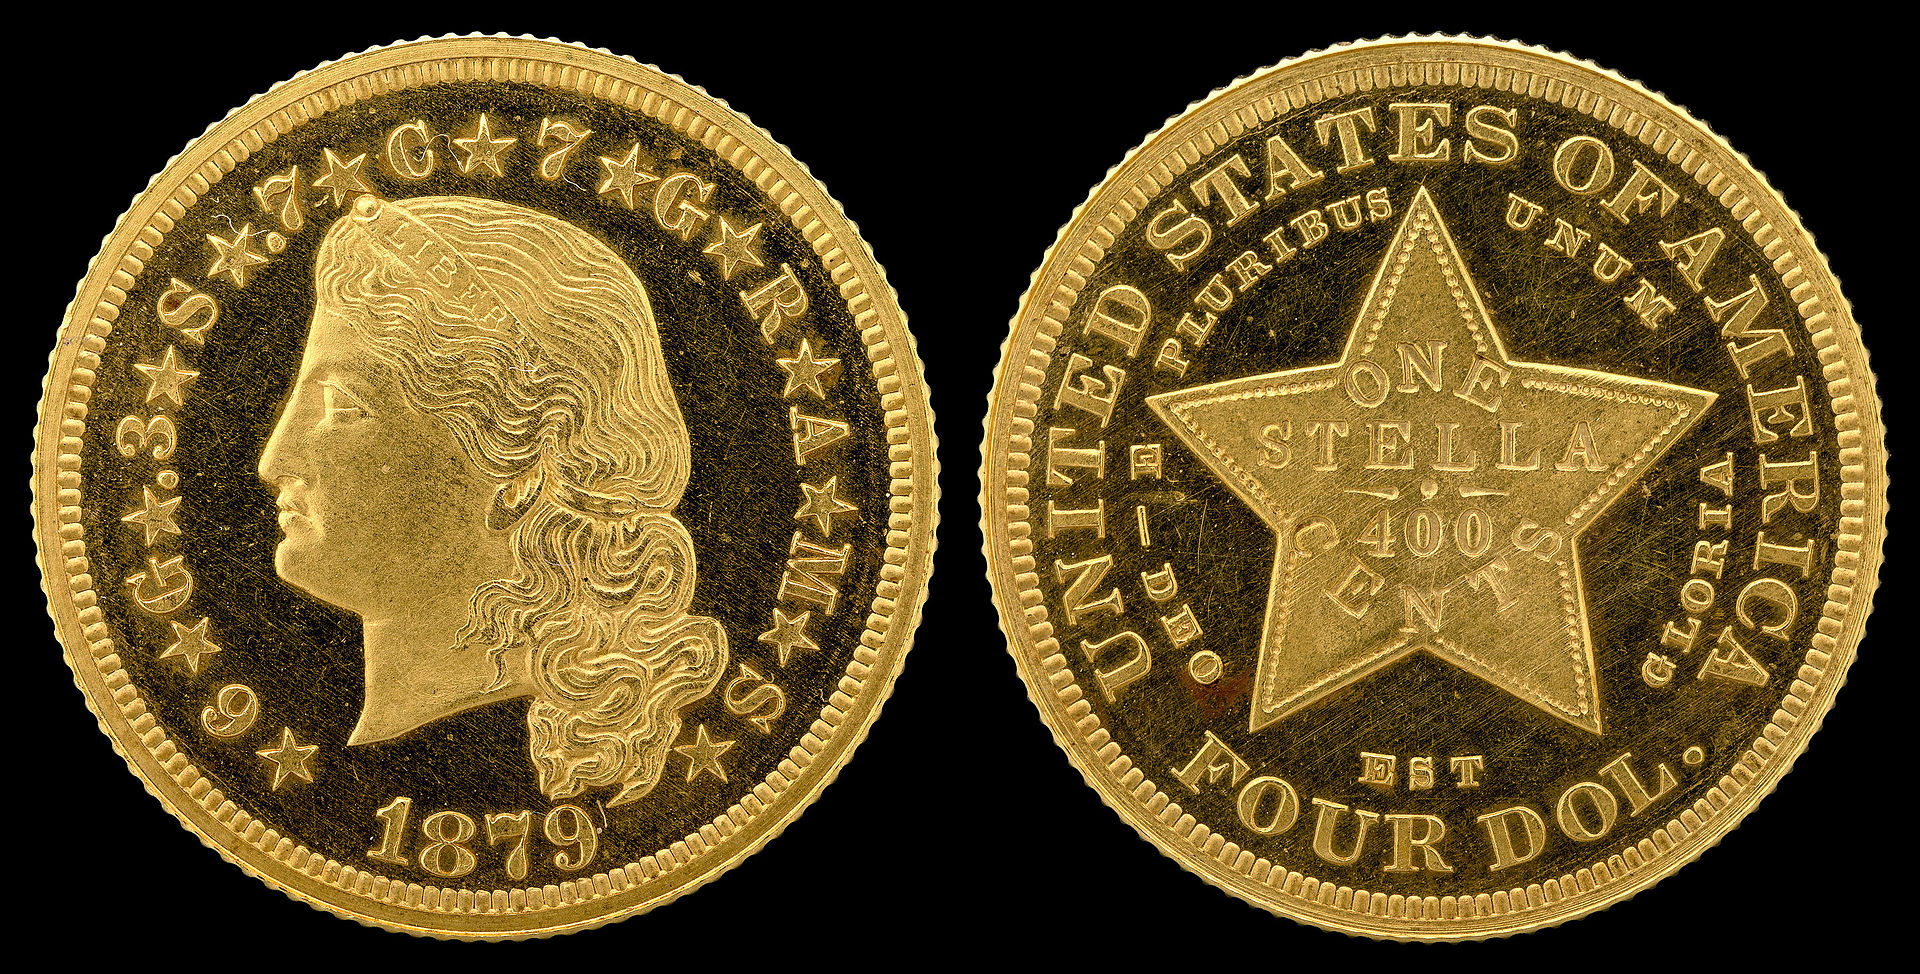
\includegraphics[width=1.0\textwidth]{4Dollar.jpg}
        \caption{4-Dollarmünze \enquote{Stella}}
        \label{subfig:4Dollar}
    \end{subfigure}
    \begin{subfigure}[b]{0.45\textwidth}
        \centering
        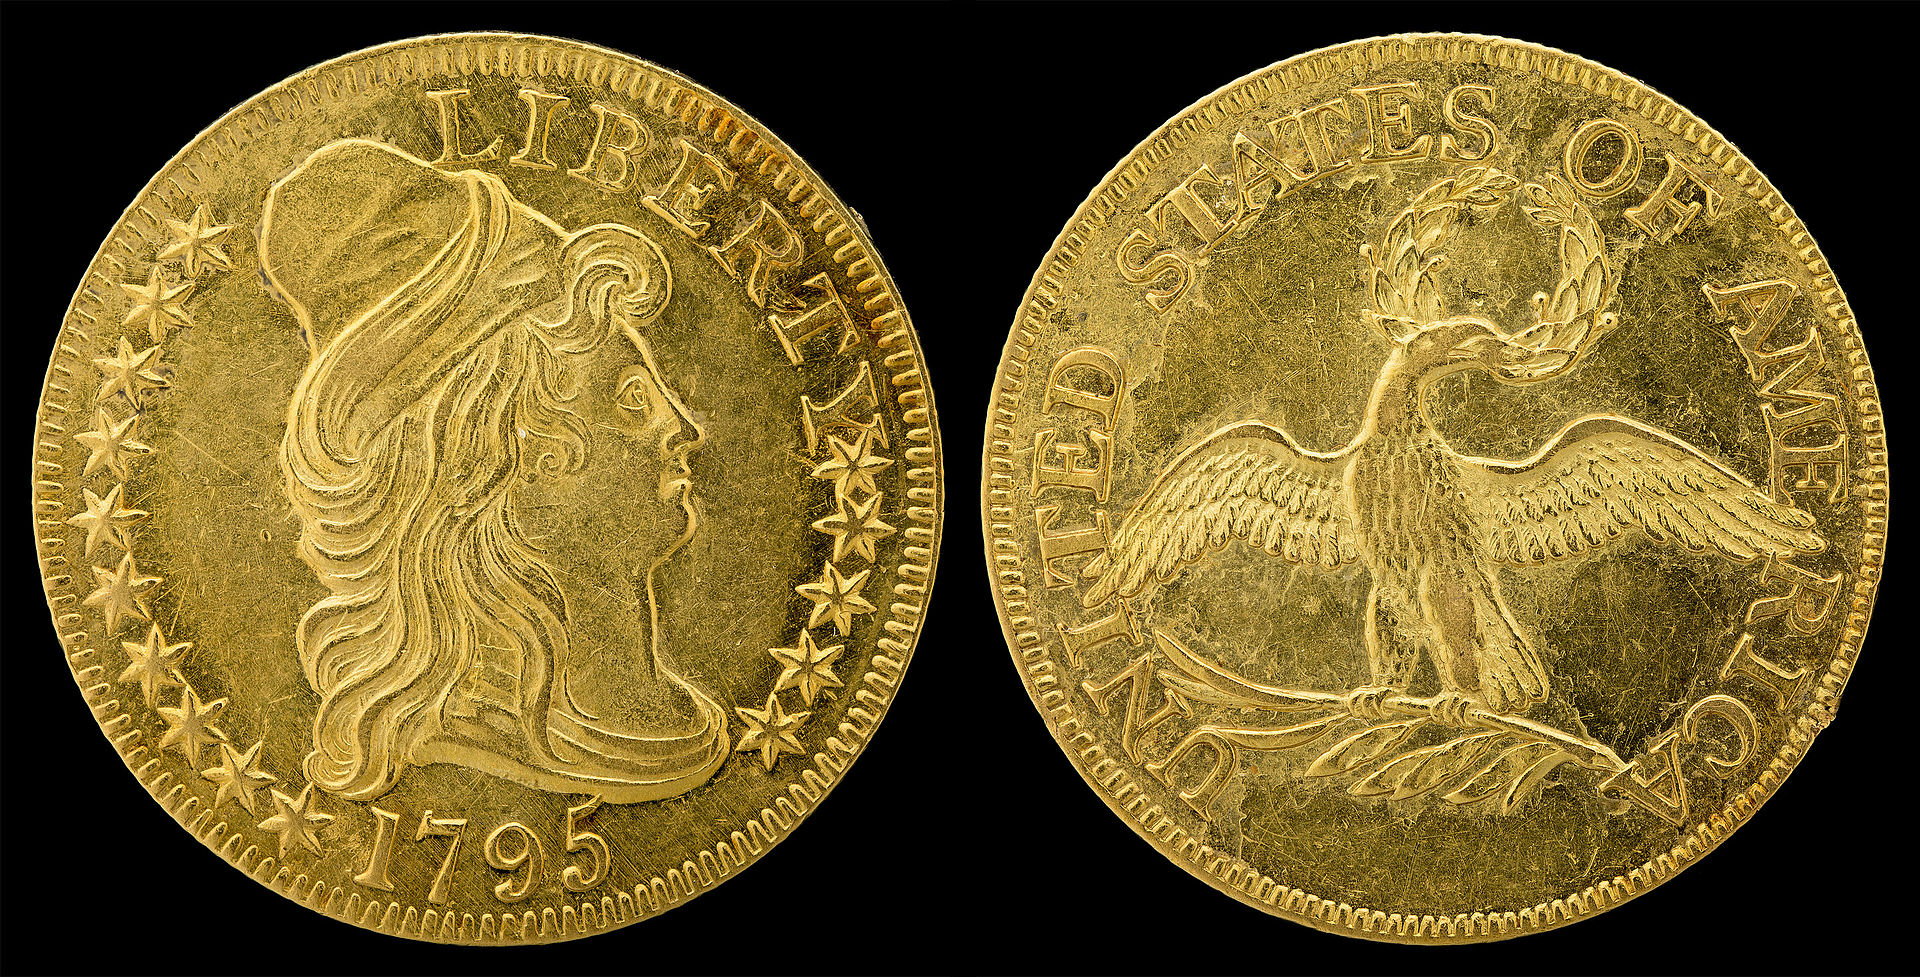
\includegraphics[width=1.0\textwidth]{5Dollar.jpg}
        \caption{5-Dollarmünze \enquote{half eagle}}
        \label{subfig:5Dollar}
    \end{subfigure}
    \caption{US-amerikanische 4-Dollarmünze und 5-Dollarmünze}
    \label{fig:Coins}
\end{figure}
\noindent
Doug findet es schade, dass diese Münzen nicht mehr geprägt werden. Schliesslich liesse sich jeder ganzzahlige Dollar-Betrag, der grösser als 11 Dollar ist, alleine durch eine Kombination dieser beiden Münzen auszahlen. Dies natürlich nur unter der Annahme, dass beliebig viele Exemplare von beiden Münzen zur Verfügung stehen.

Als kritische Menschen, sind wir nicht bereit, Doug einfach so zu glauben. Um Dougs Behauptung zu überprüfen, verwenden wir die starke Induktion (\cref{satz:starkeInduktion}). Wir definieren für jedes $n\in\N$ die Aussage $\mathcal{A}(n)$ als
\begin{center}
    $\mathcal{A}(n) :\iff $ \enquote{Der Dollar-Betrag $n$ kann durch eine Kombination aus 4-Dollarmünzen und 5-Dollarmünzen ausbezahlt werden.}
\end{center}
Dougs Behauptung besagt also, dass $\mathcal{A}(n)$ für jedes $n\in\N$ mit $n\geq 12$ gilt.

Der Betrag $n_0 = 12$ kann wegen $12 = 3\cdot 4 + 0\cdot 5$ durch drei 4er und null 5er ausbezahlt werden. Somit stimmt $\mathcal{A}(n_0)=\mathcal{A}(12)$. Zum Nachweis von $\mathcal{A}(n_0+1)=\mathcal{A}(13)$ dürften wir $\mathcal{A}(12)$ verwenden. Zum Nachweis von $\mathcal{A}(14)$ dürften wir $\mathcal{A}(12)$ und $\mathcal{A}(13)$ verwenden und zum Nachweis von $\mathcal{A}(15)$ gar $\mathcal{A}(12), \mathcal{A}(13)$ und $\mathcal{A}(14)$. Wir sehen jedoch sofort, dass
\begin{align*}
    13 &= 2\cdot 4 + 1\cdot 5, \quad 14 = 1\cdot 4 + 2\cdot 5, \quad 15 = 0\cdot 4 + 3\cdot 5
\end{align*}
und somit sind nebst $\mathcal{A}(12)$ auch $\mathcal{A}(13), \mathcal{A}(14)$ und $\mathcal{A}(15)$ nachgewiesen.

Sei nun $n\in\N$ mit $n\geq 15$. Wir beweisen, dass aus der Richtigkeit von $\mathcal{A}(k)$ für $12\leq k \leq n$ die Richtigkeit von $\mathcal{A}(n+1)$ folgt. Wir betrachten den Dollar-Betrag $n+1-4$. Offensichtlich gilt $12\leq n+1-4\leq n$. Gemäss (starker) Induktionsannahme kann der Betrag $n+1-4$ aber durch eine Kombination aus 4-Dollarmünzen und 5-Dollarmünzen ausbezahlt werden. Dies ist Aussage $\mathcal{A}(n+1-4) = \mathcal{A}(n-3)$. Durch das Hinzufügen einer einzigen 4-Dollarmünze zu dieser Kombination, erhalten wir eine gewünschte Auszahlung des Dollar-Betrags $n+1$.
}

\begin{aufgabe}{aufgabe:0208}
(*) Diese Aufgabe bezieht sich auch \cref{beispiel:Coins}. Schreiben Sie ein einfaches Python-Programm, welches für einen gegebenen ganzzahligen Dollar-Betrag $n\geq 12$ sämtliche möglichen Auszahlungen durch 4-Dollarmünzen und 5-Dollarmünzen ausgibt.

\noindent
Tipp: Verwenden Sie eine geschachtelte Schleife (eine Doppel-Schleife).
\end{aufgabe}
\begin{antwort}{aufgabe:0208}
\begin{lstlisting}[language=Python,caption=Dollar-Betrag auszahlen]
import math

def pay(n):
    combs = []
    amax = int(math.ceil(n / 4)) + 1
    bmax = int(math.ceil(n / 5)) + 1
    for a in range(amax):
        for b in range(bmax):
            if (4*a + 5*b) == n:
                combs.append((a,b))
    return combs
\end{lstlisting}
\end{antwort}

\noindent
Wir sind noch ein Beweis von \cref{satz:starkeInduktion} schuldig:

\beweis{
Wir beweisen \cref{satz:starkeInduktion}. Angenommen der Satz sei falsch und somit $\mathcal{A}(n)$ nicht jedes $n\geq n_0$ richtig. Dann ist die Menge
\begin{align*}
    N := \setct{n\in\N}{$n\geq n_0$ und $\mathcal{A}(n)$ ist falsch}
\end{align*}
nichtleer. Gemäss \cref{satz:MinimumN} besitzt die Menge $N$ ein minimales Element $m$. Da $\mathcal{A}(n_0)$ wegen Bedingung (i) richtig ist, muss $m>n_0$ gelten. Es existiert eine eindeutige natürliche Zahl $n$ mit $n+1 = m$. Aufgrund der Definition von $m$ gilt, dass die Aussagen $\mathcal{A}(k)$ für alle natürlichen Zahlen $k$ mit $n_0\leq k\leq n$ richtig sind. Dann garantiert Bedingung (ii) aber die Richtigkeit von $\mathcal{A}(n+1) = \mathcal{A}(m)$. Doch dies ist nach der Definition von $m$ unmöglich und wir haben einen Widerspruch gefunden.
}

\begin{aufgabe}{aufgabe:0210}
Der junge Tim besitzt beliebig viele Holzklötze der Länge 7 und beliebig viele der Länge 8. Klötze anderer Längen hat er keine.
\begin{aenum}
    \item Tim weiss, dass sein Plüschkrokodil die Länge 38 hat. Nun möchte er mit seinen Klötzen eine Strecke derselben Länge bauen. Doch bislang blieben alle seine Versuche erfolglos. Helfen Sie Tim, indem Sie ein Python-Programm schreiben, welches Ihnen angibt, wie viele Klötze der Länge 7 und wie viele der Länge 8 benötigt werden, um die Strecke zu bauen.
    \item Weisen Sie nach, dass es mit Tims Klötzen nicht möglich ist, eine Strecke der Länge 41 zu bauen. Schreiben Sie dazu ein Python-Programm, welches alle denkbaren Möglichkeiten ausprobiert.
    \item Beweisen Sie mit Hilfe von \cref{satz:starkeInduktion} zur starken Induktion, dass jede Strecke der Länge $n\in\N$ mit $n\geq 42$ mit Tims Klötzen gebaut werden kann.
\end{aenum}
\end{aufgabe}
\begin{antwort}{aufgabe:0210}
\begin{aenum}
    \item Das entsprechende Programm ist in \cref{listing:tim} gegeben.
\begin{lstlisting}[language=Python,caption=Bauklötze,label=listing:tim]
import math

def klotz(n):
    combs = []
    amax = int(math.ceil(n / 7)) + 1
    bmax = int(math.ceil(n / 8)) + 1
    for a in range(amax):
        for b in range(bmax):
            if (7*a + 8*b) == n:
                combs.append((a,b))
    return combs

print(klotz(38))
print(klotz(41))
\end{lstlisting}
    \item siehe (a)
    \item
Wir definieren für jedes $n\in\N$ die Aussage $\mathcal{A}(n)$ als
\begin{center}
    $\mathcal{A}(n) :\iff $ \enquote{Die Strecke der Länge $n$ kann durch eine Kombination aus Klötzen der Längen 7 und 8 gebaut werden.}
\end{center}
Die Strecke $n_0 = 42$ kann wegen $42 = 6\cdot 7 + 0\cdot 8$ gebaut werden. Somit stimmt $\mathcal{A}(n_0)=\mathcal{A}(42)$. Zum Nachweis von $\mathcal{A}(n_0+1)=\mathcal{A}(43)$ dürften wir $\mathcal{A}(42)$ verwenden. Zum Nachweis von $\mathcal{A}(44)$ dürften wir $\mathcal{A}(42)$ und $\mathcal{A}(43)$ verwenden und zum Nachweis von $\mathcal{A}(45)$ gar $\mathcal{A}(42), \mathcal{A}(43)$ und $\mathcal{A}(44)$, und so weiter. Wir sehen jedoch sofort, dass
\begin{align*}
    43 &= 5\cdot 7 + 1\cdot 8, \quad 44 = 4\cdot 7 + 2\cdot 8, \quad 45 = 3\cdot 7 + 3\cdot 8 \\
    46 &= 2\cdot 7 + 4\cdot 8, \quad 47 = 1\cdot 7 + 5\cdot 8, \quad 48 = 0\cdot 7 + 6\cdot 8
\end{align*}
und somit sind nebst $\mathcal{A}(42)$ auch $\mathcal{A}(s)$ für $s\in\lrc{43,44,45,46,47,48}$ nachgewiesen.

Sei nun $n\in\N$ mit $n\geq 48$. Wir beweisen, dass aus der Richtigkeit von $\mathcal{A}(k)$ für $42\leq k \leq n$ die Richtigkeit von $\mathcal{A}(n+1)$ folgt. Wir betrachten die Strecke der Länge $n+1-7$. Offensichtlich gilt $42\leq n+1-7\leq n$. Gemäss (starker) Induktionsannahme kann die Strecke der Länge $n+1-7$ aber durch eine Kombination aus Klötzen der Längen 7 und 8 gebaut werden. Dies ist Aussage $\mathcal{A}(n+1-7) = \mathcal{A}(n-6)$. Durch das Ansetzen eines Klotzes der Länge 7 zu dieser Kombination, erhalten wir eine Strecke der Länge $n+1$.
\end{aenum}
\end{antwort}

\begin{aufgabe}{aufgabe:0310}
Seien $+$ und $\cdot$ assoziative und kommutative Verknüpfungen auf einer Menge $X$, welche das Distributivgesetz:
\begin{align*}
    (x+y)\cdot z = x\cdot z + y\cdot z
\end{align*}
für $x,y,z\in X$ erfüllen. Beweisen Sie mit Hilfe von \cref{satz:starkeInduktion} zur starken Induktion die Richtigkeit des \enquote{verallgemeinerten} Distributivgesetztes:
\begin{align*}
    \mathcal{A}(n) :\iff c\sum_{k=0}^n\lr{x_k} = \sum_{k=0}^n\lr{cx_k}
\end{align*}
für alle $n\in\N$. Dabei sind $c\in X$ und $(x_k)$ eine Folge in $X$. 
\end{aufgabe}
\begin{antwort}{aufgabe:0310}
Aussage $\mathcal{A}(0)$ ist offensichtlich richtig.

Wir zeigen nun, dass aus der Richtigkeit von $\mathcal{A}(k)$ für $0\leq k\leq n$ die Richtigkeit von $\mathcal{A}(n+1)$ folgt. Dazu betrachten wir:
\begin{align*}
    &c\sum_{k=0}^{n+1}\lr{x_k} = \\
    &c\lr{x_{n+1} + \sum_{k=0}^{n}\lr{x_k}} \stackrel{\text{Distributivgesetz}}{=} \\
    &cx_{n+1} + c\sum_{k=0}^{n}\lr{x_k} \stackrel{\text{Induktionsvoraussetzung}}{=} \\
    &cx_{n+1} + \sum_{k=0}^{n}\lr{cx_k} = \\
    &\sum_{k=0}^{n+1}\lr{cx_k}.
\end{align*}
Mit dem Prinzip der starken Induktion folgt somit, die Richtigkeit der Aussage $\mathcal{A}(n)$ für alle $n\in\N$.
\end{antwort}

% 4-Dollar Stella
% US Mint (coin), National Numismatic Collection (photograph by Jaclyn Nash) - National Numismatic Collection, National Museum of American History
% 5-Dollar half eagle
% US Mint (coin), National Numismatic Collection (photograph by Jaclyn Nash) - National Numismatic Collection, National Museum of American History
\clearpage
\shipoutAnswer